% !Tex root = checkedc.tex

\chapter{Bounds for variables}
\label{chapter:tracking-bounds}

Variable with \arrayptr\ types that are used to access
memory must have bounds declared for them.  The same requirement
holds for variables with incomplete checked array types.

For an \arrayptr\ variable, the bounds will be used to check
memory accesses at runtime involving the pointers stored in the variable
or pointers produced by pointer arithmetic that uses those pointers.
Runtime checks can be omitted if a compiler proves that they are
redundant. In addition, for performance-critical code, checks will be
omitted when programmers demonstrate at compile-time that the checks are
redundant (see Section~\ref{section:avoiding-bounds-checks} for details).

\section{Bounds declarations}
\label{section:bounds-declarations}

Bounds are declared using bounds declarations. Bounds declarations have
the form:

\begin{tabbing}
\var{bounds}\=-\var{decl:} \\
\> \boundsdecl{\var{x}}{\var{bounds-exp}} \\
\\
\var{bounds}\var{-exp:} \\
\> \texttt{count(}\var{non-modifying-exp}\texttt{)} \\
\> \bounds{\var{non-modifying-exp}}{\var{non-modifying-exp}} \\
\> \boundsnone \\
\> \boundsany
\end{tabbing}

where \var{x} is a variable. There are additional forms for handling
casts and void pointers that are described in 
Sections~\ref{section:pointer-cast-results} and \ref{section:pointers-to-void}.

A bounds expression describes the memory that can be accessed using the
value of \var{x}, provided that x is not null. Bounds expressions
include counts, pairs that specify an upper bound and lower bound,
\boundsnone, and \boundsany:

\begin{itemize}
\item
  \boundsdecl{\var{x}}{\boundscount{e1}} describes the number of
  elements that are accessible beginning at \var{x}. Only memory that
  is at or above x and below \var{x} \texttt{+} \var{e1} can be
  accessed through \var{x}, where \var{x} \texttt{+} \var{e1} is
  interpreted using \arrayptr\ pointer arithmetic.
\item
  \boundsdecl{\var{x}}{\bounds{\var{e1}}{\var{e2}}}
  describes the range of memory that can be accessed through \var{x}.
  Only memory that is at or above the location specified by \var{e1}
  and below \var{e2} can be accessed through \var{x}.
\item
  \boundsdecl{\var{x}}{\boundsnone} declares that \var{x} has no bounds.
  It is an error at compile-time to attempt to access memory using a
  variable of type \arrayptr\ with no bounds.
\item
  \boundsdecl{\var{x}}{\boundsany} is a special form that readers can
  ignore for now. It is used for null pointers (0 cast to a pointer
  type) and means that \var{x} can have any bounds. Because null
  pointers cannot be used to access memory, they can have any bounds.
\end{itemize}

Bounds expression use ``non-modifying'' expressions. These are a subset
of C expressions that do not modify variables or memory. They include
local variables, parameters, constant expressions, casts, and operators
such as addition, subtraction, and address-of. 
Section~\ref{section:non-modifying-expressions}  describes
non-modifying expressions in detail.

In a bounds declaration of the form \boundsdecl{\var{x}}{\var{bounds-exp}},
\var{x} must have an \arrayptr\ or a checked array type. 
For the form  \boundsdecl{\var{x}}{\boundscount{\var{e1}}},  the type of 
\var{x} cannot be \arrayptrvoid\ and the type of \var{e1} must be an integral type. 
For \boundsdecl{\var{x}}{\bounds{\var{e1}}{\var{e2}}}, \var{e1} and
\var{e2} must have the same \arrayptr\ type. The type of x is
typically the same type as \var{e1} and \var{e2}, but it can be a
different \arrayptr\ or checked array type. Allowing the types
to be different is useful for describing the results of pointer casts and
bounds for \arrayptrvoid\ pointers.

For any variable with a bounds declaration, the variable must be
non-null when memory is accessed There is no requirement that an
\arrayptr\ variable stay within its bounds. The requirement is
that the \arrayptr\ variable can only be dereferenced if it is
in bounds. This avoids bound checks on pointer arithmetic.

Count expressions have limits on their ranges to prevent signed integer
overflow and unsigned integer wraparound from affecting size
computations. Section~\ref{section:integer-overflow-informal}
explains these limits in detail. The limits
depend on the element type of the \arrayptr\ and the type of the count
expression. For \boundsdecl{\var{x}}{\boundscount{\var{e1}}}, where \var{x}
has type \arrayptrT ,
\var{e1} must be greater than or equal to 0. \var{e1} must be less
than the maximum number of an
\arrayptrT\ elements
that can be indexed by an integer whose type matches that of \var{e1}.
A bounds declaration \boundsdecl{\var{x}}{\boundscount{\var{e1}}} is an
abbreviation for \boundsdecl{\var{x}}{\bounds{\var{x}}{\var{x} \texttt{+} \var{e1}}} with additional conditions that \var{e1}
\texttt{>= 0 \&\& \var{e1} <= (char *)}
\var{ub}\texttt{.} \var{ub} is either
\texttt{UINTPTR\_MAX/\sizeof{\var{T}}} or
\texttt{INTPTR\_MAX/\sizeof{\var{T}}}. 

The conditions may require programmers to add additional checks at memory allocations
to show that \var{e1} is in range. However, the conditions have advantages too.
They provide scaffolding for proving that expressions based on
element counts of \arrayptr\ variables do not overflow or wraparound.

The meaning and correctness of bounds are based on the C semantics for
pointers and pointer arithmetic. At runtime, any non-null pointer in C
has an object associated with it. The association starts when a pointer
is created by a memory allocation operation, address-of expression, or
conversion of an array variable to a pointer-typed expression. It flows
through to pointers that result from pointer arithmetic. At runtime, the
bounds for a pointer must be the bounds of the object associated with
the pointer or a subrange of those bounds. The correctness of declared
bounds information at compile-time is ensured by making allocation sites
and address-of expressions be creators of bounds information and by
propagating bounds with the pointers with which they are associated.
Bounds can be narrowed during propagation, but they cannot be widened.

The meaning of a bounds expression can be defined more precisely. At
runtime, given an expression \var{e} with a bounds expression
\bounds{\var{lb}}{\var{ub}}, let the runtime
values of \var{e}, \var{lb}, and \var{ub} be \var{ev}, \var{lbv},
and \var{ubv}, respectively. The value \var{ev} will be \texttt{0} (null) or
have been derived via a sequence of operations from a pointer to some
object \var{obj} with \bounds{\var{low}}{\var{high}}.
The following statement will be true at runtime:
\var{ev} \texttt{== 0 || (\var{low} <= \var{lbv}\&\& 
\var{ubv} <= \var{high})}. In other words, 
if \var{ev} is null, the bounds
may or may not be valid. If \var{ev} is non-null, the bounds must be
valid. This implies that any access to memory where \var{ev} \texttt{!=
0 \&\&} \var{lbv} \texttt{<=} \var{ev} \texttt{\&\&} \var{ev}
\texttt{<} \var{ubv} will be within the bounds of \var{obj}.

In this section, to simplify the description, it is assumed that none of
the \arrayptr\ variables that have bounds declarations have
their addresses taken. It is also assumed that the values of variables
whose addresses are taken are not used in bounds declarations. It is
acceptable to use the address of an address-taken variable in a bounds
declaration. This is provided that the resulting address is not used to
access memory in the bounds declaration (that is, indirectly access the
value of a variable). For example, given the declaration \texttt{int x},
the expression \texttt{\&x} may appear in a bounds expression.  
Chapter~\ref{chapter:pointers-to-data-with-arrayptrs} extends the
design to avoid these restrictions.  It covers pointers to data with 
\arrayptr\ values,  pointers to variables used in bounds, and bounds 
that use pointers.

\subsection{Using bounds declarations}

Bounds declarations may be added to declarations and statements using
\keyword{where} clauses. They also may be placed inline at a declaration
by following the declarator with \texttt{:} \var{bounds-exp}. In that
case, the bounds expression applies to the variable that is the subject
of the declarator. By making the bounds be part of the program, this
preserves the control and efficiency of C. The bounds declarations will
be checked statically for correctness using rules described in 
Chapter~\ref{chapter:checking-bounds}.

\subsection{Bounds declarations at variable declarations}
\label{section:variable-declarations}

Here are some examples of bounds declarations as part of variable
declarations. The first function sums the integers stored in memory
between \texttt{start} and \texttt{end}, where the integer stored at
\texttt{end} is not included.

\begin{verbatim}
int sum(array_ptr<int> start : bounds(start, end), array_ptr<int> end)
{ 
    int result = 0;
    array_ptr<int> current : bounds(start, end) = start;
    while (current < end) {
       result += *current++; // *current is bounds-checked.  The checking ensures 
                             // that current is within the bounds of (start, end) 
                             // at the memory access.                           
    }
    return result;
}
\end{verbatim}

This can be written using \keyword{where} clauses as well, at the
inconvenience of typing variable names twice in declarations:

\begin{verbatim}
int sum(array_ptr<int> start where start : bounds(start, end), array_ptr<int> end)
{ 
    int result = 0;
    array_ptr<int> current where current : bounds(start, end) = start;
    while (current < end) {
       result += *current++;                          
    }
    return result;
}
\end{verbatim}

This function searches for an integer in an array. If it finds the
integer, it returns the index in the array where the integer occurs.
Otherwise, it returns -1.

\begin{verbatim}
int find(int key, array_ptr<int> a : count(len), int len)
{
    for (int i = 0; i < len; i++) {
         if (a[i] == key) { // a[i] is bounds checked.  The checking
                            // ensures that i is between 0 and len.
             return i;
         }
    }
    return -1;
}
\end{verbatim}

If the code was written assuming that it would always find the integer,
bounds-checking would detect the buffer overrun in the case the integer
was not present:

\begin{verbatim}
int bad_find(int key, array_ptr<int> a : count(len), int len)
{
    int i = 0;
    while (1) {
        if (a[i] == key) { // The bounds check will fail when i == len
            return i;
        }
        i++;
    }
    return -1;
}

\end{verbatim}

This function adds two arrays of 2x2 arrays.

\begin{verbatim}
int add(int a checked[][2][2] : count(len), int b checked[][2][2] : count(len), 
        int len) 
{
    for (int i = 0; i < len; i++) {
        // All array accesses are bounds checked
        a[i][0][0] += b[i][0][0]; 
        a[i][0][1] += b[i][0][1];
        a[i][1][0] += b[i][1][0];
        a[i][1][1] += b[i][1][1];
    }
}
\end{verbatim}

Externally-scoped variables can have bounds as well:

\begin{verbatim}
// external-scoped variables that hold a buffer and its length
int buflen = 0;
array_ptr<int> buf : count(buflen) = NULL;

int sum()
{
    int result = 0;
    for (int i = 0; i < buflen; i++) {
        result += buf[i]; // bounds checked
    }
    return result;
}
\end{verbatim}

This is a declaration of a function that copies bytes provided that the
pointers and lengths are aligned:
\begin{verbatim}
int aligned_memcpy(array<char> dest where dest : count(len) && aligned(dest, 4),
                   array<char> src where src : count(len) && aligned(src, 4),
                   int len where len % 4 == 0);
\end{verbatim}

The declaration can be shortened using in-line bounds declarations to:

\begin{verbatim}
int aligned_memcpy(array<char> dest : count(len) where aligned(dest, 4),
                   array<char> src : count(len) where aligned(src, 4),
                   int len where len % 4 == 0);
\end{verbatim}

This example is adapted from the OpenSSL library. The signature of a
method has been modified to have bounds declaration. The size of input
and output buffers must be multiples of 16 because the function operates
on 16-byte chunks of data.

\begin{verbatim}
void AES_cbc_encrypt(array_ptr<const unsigned char> in : count(len),
                     array_ptr<unsigned char> out : count(len),
                     size_t len where len % 16 == 0,
                     ptr<const AES_KEY> key,
                     array_ptr<unsigned char> ivec : count(16),
                     const int enc);
\end{verbatim}

\subsection{Bounds declarations at expression statements}
\label{section:statement-declarations}

Programmers may wish to delay initializing variables or may wish to
change the bounds of a variable in the middle of a function. This can be
done using bounds declarations attached to expression statements. In C,
an expression is converted to a statement by placing a semi-colon after
the expression. This creates an expression statement. A \keyword{where}
clause may be added before the terminating semi-colon of an expression
statement.

Any variable that has bounds declared at an expression statement has
dataflow-sensitive bounds throughout the body of the function. Only
automatic variables can have bounds declared for them at expression
statements. It does not make sense to have dataflow-sensitive bounds for
externally-scoped variables and variables with static or thread storage.
The bounds extend to the next assignment to any variable in the bounds
declaration, with some exceptions for pointer incrementing or
decrementing. Section~\ref{section:extent-of-declarations} 
describes the extent of flow-sensitive bounds
in more detail.

Here is a simple example that illustrates bounds declarations at
statements. The variable \texttt{tmp} first points to an array with 5
elements and then points to an array with 10 elements; the bounds are
adjusted accordingly.

\begin{verbatim}
void f() 
{
   int x[5];
   int y[10];
   array_ptr<int> tmp;
   tmp = x where tmp : count(5);
   ...
   tmp = y where tmp : count(10);
}
\end{verbatim}

In the second example, an \arrayptr\ \texttt{c} and its length are initialized
lazily to either \texttt{a} or \texttt{b}, depending on another parameter \texttt{val}:

\begin{verbatim}
/* use either a or b depending on val */
int choose(int val, array_ptr<int> a : count(alen), int alen,
                    array_ptr<int> b : count(blen), int blen) 
{
    array_ptr<int> c ;
    int clen;
    if (val) {
        clen = alen;
        c = a
        where c : count(clen);
    }
    else {
        clen = blen;
        c = b
        where c : count(clen);
    }    
    ...
}
\end{verbatim}

Declaring bounds at assignments supports updating of variables that are
used in the bounds for an existing \arrayptr\ variable. New
bounds for the \arrayptr\ variable can be declared to reflect
the update. Consider the following example:

\begin{verbatim}
/* sum integers stored between start and end, where end is not included */
int sum(array_ptr<int> start : bounds(start, end), array_ptr<int> end)
{ 
    ...
    // Adjusting end. Can declare new bounds for start at the assignment
    end = end - 1 where start : bounds(start, end + 1);
}
\end{verbatim}

\subsubsection{Bounds declarations for return values}

Bounds may be declared for the value returned by a function. The
parameter list can be followed by either \texttt{:} \var{bounds-exp} or
a \keyword{where} clause. The special variable \keyword{return\_value} can
be used to refer to the return value. The parameters are considered in
scope for the bounds declaration or \keyword{where} clause. Any parameters
occurring in the return bounds declaration or \keyword{where} clause may
not be modified by the body of the function.

The following example show the \texttt{find} function from
Section~\ref{section:variable-declarations} modified
to return a pointer to the element instead of the index:

\begin{verbatim}
array_ptr<int> find(int key, array_ptr<int> a : count(len), int len)
 : bounds(a, a + len)
{
    for (int i = 0; i < len; i++) {
         if (a[i] == key) { // a[i] is bounds checked.  The checking
                            // ensures that i is between 0 and len.
             return &a[i];
         }
    }
    return NULL;
}
\end{verbatim}

This also can be written as:

\begin{verbatim}
array_ptr<int> find(int key, array_ptr<int> a : count(len), int len)
  where return_value : bounds(a, a + len)
{
   ...
}
\end{verbatim}
Here is the declaration of a function that allocates memory:

\begin{verbatim}
array_ptr<char> alloc(size_t size) : count(size);
\end{verbatim}

\subsection{Invariant bounds declarations}
\label{section:invariant-bounds-declarations}

Variables that only have bounds declared for them at their definition
have bounds that are invariants. Any assignments to the variable
\emph{or} variables in the bounds expression must maintain the
invariant. The invariant can be suspended temporarily during updates.

Because externally-scoped \arrayptr\ variables can have bounds declared
for them only at their definitions, by definition their bounds are
always invariants.

\subsection{Lexical hiding of variables}

A nested lexical scope is not allowed to hide a variable used in a
bounds declaration within the extent of the bounds declaration. This
prevents programs from accidentally invalidating the bounds declaration:

\begin{verbatim}
/* illegal function */
void bad(int i) 
{
    array_ptr<int> x : count(i) = malloc ((sizeof(int) * i);
    {
        int x = 5;     // hide x
        i = INT_MAX;   // subvert bounds
    }
    x[random()] = 0xbad;
}
\end{verbatim}

\subsection{Storage class-related requirements}

Local variables with static storage class or thread storage class can
have only bounds declarations with bounds expressions that use variables
with the same storage class as the local variable or variables that are declared
\texttt{const}. The memory for static variables and thread variables
persists across exit and reentry from functions and blocks. It follows
that the bounds information must persist also.

Local variables with automatic storage class can have bounds
declarations with bounds expressions that use variables with automatic,
static, or thread storage class. However, the extent of local variable
bounds declarations that use variables with external linkage ends at
function calls, unless the variables with external linkage are declared
\texttt{const}. This is because the function calls may modify the
variables with external linkage.

\section{Variables at external scope}
\label{section:external-scope-variables}

If there are multiple declarations of a variable with external scope in
a translation unit, the bounds declaration and/or \keyword{where} clauses for the
variable must be identical at all the declarations. This prevents the
specification of different bounds for global variables in the same
compilation unit. Any variables with external scope that have bounds
declarations and/or \keyword{where} clauses must have the same bounds declaration
and where clauses in all translation units.

All places in a program that may write to a variable with external scope
also must have the same view of the bounds declarations involving that
variable. This allows static checking to ensure that bounds declarations
remain valid.

To see what can go wrong without this requirement, consider the
following example:

\begin{verbatim}
extern int size;

void update_size(int i)
{
    num = i;
}

extern array_ptr<int> ap : count(size);

void go()
{
    update_size(INT_MAX);
    ap[100] = 0xbad;
}

// define size and ap
int size = 10;
int arr[10];
array_ptr<int> ap = arr : count(size);
\end{verbatim}

The checking of bounds declarations does not know at
\texttt{update\_size} that \texttt{ap} needs to have at least \texttt{i}
elements when \texttt{size} is updated, allowing a programmer to accidentally
invalidate bounds declarations.

A simple rule enforces this restriction. Given the initial declaration
in a translation unit of a variable with external scope that has a
\keyword{where} clause, there cannot be any function definitions between
the declaration and the initial declarations of other variables used in
the bounds declaration for the variable or the optional \keyword{where} clause for the declaration.
It is possible for the initial declaration of
a variable with external scope to occur within the body of a function.
In that case, there cannot be any statements or declarations of
non-external variables with initializers between the initial declaration
and the initial declarations of other variables used in the
bounds declaration for the variable or the optional \keyword{where} clause for
the declaration.

\section{Syntax changes}
The grammar from the ``C Programming Language'' \cite{Ritchie1988} is extended to include
in-line bounds declarations and \keyword{where} clauses for declarations:

\begin{tabbing}
\var{init-}\=\var{declarator:} \\
\>\var{declarator inline-bounds-specifier\textsubscript{opt} where-clause\textsubscript{opt}} \\
\>\var{declarator inline-bounds-specifier\textsubscript{opt} 
where-clause\textsubscript{opt}} \texttt{=} \var{initializer
where-clause\textsubscript{opt}} \\
\>\ldots{} \\
\\
\var{parameter-declaration:} \\
\>\var{declaration-specifiers declarator} \var{inline-bounds-specifier\textsubscript{opt} where-clause\textsubscript{opt}} \\
\\
\var{inline-bounds-specifier:}\\
\>\texttt{:} \var{bounds-exp} \\ 
\\
\var{where-clause}: \\
\>\keyword{where} \var{facts} \\
\\
\var{facts:} \\
\>\var{fact} \\
\>\var{fact} \texttt{\&\&} \var{facts} \\
\\
\var{fact:}\\
\>\var{variable inline-bounds-specifier} \\
\>\var{variable relop non-modifying-exp} \\
\>\var{non-modifying-exp relop variable} \\
\\
where \var{relop} is one of \verb|<|, \verb|<=|, \verb|==|,
\verb|!=|, \verb|>=|, \verb|>|.\\
\\
In addition, the grammar is updated to allow where clauses at expression
statements:\\
\\
\var{expression-statement:}\\
\>\var{expression\textsubscript{opt} where-clause\textsubscript{opt}}\texttt{;}
\end{tabbing}

\section{Operations allowed in non-modifying expressions}
\label{section:non-modifying-expressions}

As mentioned earlier, non-modifying expressions are a subset of C
expressions that do not modify variables or memory. The subexpressions
of a non-modifying expression must themselves be non-modifying
expressions. Non-modifying expressions include the following kinds of
expressions:

\begin{compactitem}
\item
  Local variables and parameter variables
\item
  Constant expressions
\item
  Cast expressions
\item
  Address-of expressions
\item
  Unary plus/minus expressions
\item
  One's complement expressions
\item
  Logical negation expressions
\item
  Sizeof expressions
\item
  Multiplicative expressions (\texttt{*}, \texttt{/}, \texttt{\%})
\item
  Additive expressions (\texttt{+}, \texttt{-})
\item
  Shift expressions (\texttt{>>}, \texttt{<<})
\item
  Relational and equality expressions (\texttt{<}, \texttt{>},
  \texttt{<=}, \texttt{>=}, \texttt{==}, \texttt{!=})
\item
  Bitwise expressions: and (\texttt{\&}), or (\texttt{|}), exclusive-or (\texttt{\^})
\item
  Logical AND (\texttt{\&\&}) and logical OR (\texttt{||}) expressions
\item
  Conditional expressions
\item
  Access to special members of \spanptr\ types
  (\texttt{current}, \texttt{lower\_bound}, and \texttt{upper\_bound})
\end{compactitem}

They also include expressions that access members of types or memory:

\begin{compactitem}
\item
  Member references (to members of structures or unions) (the \texttt{.}
  operator)
\item
  Indirect member dereferences (\texttt{->})
\item
  Pointer dereferences
\end{compactitem}

The static checking of the validity of bounds declarations restricts the
usage of non-modifying expressions that read memory when memory is being
modified.

Non-modifying expressions do not include:

\begin{compactitem}
\item
  Assignment expressions (for the reason that evaluating them repeatedly
  at bounds checks would produce unexpected results)
\item
  Pre-increment/decrement and post-increment/decrement expressions
  (these are forms of assignments)
\item
  Volatile variables
\item
  Function calls (because these may contain assignments that modify
  variables or memory)
\item
  Comma expressions (because bounds expressions do not allow side
  effects, these can always be simplified to the second expression)
\end{compactitem}

It is suggested that programmers use simple non-modifying expressions because
the expressions may be fully re-evaluated at every bounds check involving the
bounds expression. More complicated bounds expressions are allowed
because programmers might find them useful.

\section{Bounds declarations for results of casts between \arrayptr\ types}
\label{section:pointer-cast-results}

Typically \arrayptr\ pointers and their bounds are relatively
aligned. Together, they represent a view of an array of \var{T}, where
the pointer has type
\arrayptrT. The
bounds specify a range of memory that is exactly the size of some array
of T and the pointer points exactly at an element of that array. For
example, suppose short ints are 2 bytes in size and 
{\texttt{\boundsdecl{x}{\bounds{y}{z}}}}, where the types of \texttt{x},
\texttt{y}, \texttt{z} are \arrayptrinst{\texttt{short int}} .

This illustration shows 12 consecutive bytes in memory beginning at
address a\textsubscript{0}, where \texttt{y} and \texttt{z} bound a
3-element array and \texttt{x} points to the middle of the array. The
memory occuped by the 3-element array is shaded in light blue, and the
element pointed to by x is also cross-hatched. The distances in bytes
between \texttt{x}, \texttt{y}, and \texttt{z} are all multiples of 2,
the size of \texttt{short int}.
\begin{center}
\relalignpic{4}
\end{center}

This simplifies bounds checking because there is no concern during a
bounds check that a pointer will access memory at the end or beginning
of the array that partially overlaps with the bounds. Suppose, for
example, that \texttt{x} was not relatively aligned to \texttt{y} and
\texttt{z} and points at a\textsubscript{7}. The object pointed to by
\texttt{x} now straddles the array bounds. This illustration shows this:
\begin{center}
\relalignpic{7}
\end{center}

When \texttt{x} is not relatively aligned, the bounds check for x
becomes more expensive. With relative alignment, the bounds check is
\texttt{y <= x} and \texttt{x < z}. Without relative
alignment, the check for the upper bound needs to compute the highest
address that will be accessed using x. For this example, the highest
address accessed will be
\texttt{(\arrayptrchar) x + \sizeof{short int} - 1}, so the check becomes 
\texttt{y <= x} and \texttt{x + 1 < z}.

A pointer cast can create a pointer that is not relatively aligned to
the referent type of the pointer type. This can happen when:

\begin{enumerate}
\item
  A pointer is cast to be a pointer to a larger type. For example, if an
  \arrayptrinst{\texttt{short int}}\ is cast to be an
  \arrayptrint , the resulting pointer
  may not be relatively aligned to its bounds for \texttt{int}. In the
  first illustration where \texttt{x} points to a4,
  \arrayptrint\ \texttt{x} is not relatively
  aligned to \texttt{y} for \texttt{int}.
\item
  A pointer is cast to be a pointer to a smaller type, and the size of
  the original referent type is not a multiple of the size of the
  smaller type. For example, a pointer to a 12-byte struct may not be
  relatively aligned to its bounds when it is cast to a pointer to an
  8-byte struct.
\end{enumerate}

The use of struct types to illustrate the second case is intentional.
For most C implementations, the second case never happens for casts
involving scalar types. Scalar types are powers of 2 in size (1, 2, 4,
and 8 bytes). This means that for a cast from a larger scalar type to a
smaller scalar type, the larger scalar type will always be a multiple of
the smaller scalar type.

In general, an
\arrayptrT\ that is
relatively aligned for \var{T} is guaranteed to be relatively aligned
for \arrayptrinst{\textit{S}} only
when \sizeof{\var{S}} is a common factor of
\sizeof{\var{T}}. In other cases, programmers need to
supply additional information using program invariants to show that an
\arrayptr\ pointer is relatively aligned to its bounds. Of
course, programmers who are doing casts to use operations on larger
types instead of operations on smaller types (for example, \texttt{int}
instead of \texttt{char}) usually already are doing these checks.

\subsection{Representing relative alignment in bounds declarations}
\label{section:representing-relative-alignment}

Bounds expressions are extended with an optional relative alignment 
clause to represent situations where an \arrayptrT\ is not relatively 
aligned to its bounds for type \var{T}:

\begin{tabbing}
\var{bounds}\=\var{-exp:}\\
\> \var{\ldots{}}\\
\> \bounds{\var{non-modifying-exp}}{\var{non-modifying-exp}}
         \var{relative-alignment-clause\textsubscript{opt}} \\
\\
\var{relative-alignment-clause:}\\
\> \relalign{\var{type}} \\
\> \relalignval{\var{constant-exp}} 
\end{tabbing}

This clause is only added to bounds pairs because (by definition) count
expressions always describe pointers that are relatively aligned to
their bounds. The optional relative alignment clause specifies a
relative alignment type \var{T} or the required relative alignment in
bytes. Given 
\boundsdecl{\var{x}}{\boundsrel{\var{e1}}{\var{e2}}{\var{T}}},
\texttt{((\arrayptrchar) \var{x} - (\arrayptrchar) \var{e1}) \%
        \sizeof{\var{T}} == 0} and
\texttt{((\arrayptrchar) \var{e2} - (\arrayptrchar) \var{x}) \%
sizeof(\var{T}) == 0} must be true. If the number of bytes is
specified, \sizeof{\var{T}} is replaced by the
constant expression.  The relative alignment clause \relalign{\var{type}}
is just short-hand for \relalignval{\texttt{sizeof(\var{type})}}.

\subsection{Examples of uses of bounds declarations that specify relative alignment}

Here are examples of the use of relative alignment clauses in
conjunction with pointer casts. In the first example, there is an
\arrayptr\ to raw data consisting of characters. The pointer is
cast to be an \arrayptrint . However,
the relative alignment remains \texttt{char}:

\begin{verbatim}
// cast data to be an array_ptr<int> instead
array_ptr<char> raw_data : bounds(lower, upper) = ...
array_ptr<int> data : bounds(lower, upper) rel_align(char) =
    (array_ptr<int>) raw_data;
\end{verbatim}

In the second example, the code starts with an
\arrayptrint. The pointer is cast to
be an \arrayptrchar. That
\arrayptr\ is then cast back to be an
\arrayptrint . In the second cast, the
\texttt{rel\_align} clause is omitted because the default relative
alignment for an \arrayptrint\ is
\texttt{int}.

\begin{verbatim}
array_ptr<int> data : bounds(lower, upper) = ...
array_ptr<char> byte_data : bounds(lower, upper) rel_align(int) = (array_ptr<char>) data;
array_ptr<int> finish : bounds(lower, upper) = (array_ptr(int>) byte_data;
\end{verbatim}

The third example illustrates a subtlety when an
\arrayptrT\ has a
relative alignment that is larger than the actual size of \var{T}. The
use of pointer arithmetic may require that relative alignment be
lowered. Suppose that the size of \texttt{short int} is 2 bytes and the
size of an \texttt{int} is 4 bytes:

\begin{verbatim}
array_ptr<int> d : bounds(lower, upper) = ...
array_ptr<short int> e : bounds(lower, upper) rel_align(int) = (array_ptr<short int>) d;
array_ptr<short int> f : bounds(lower, upper) rel_align(short int) = e + 1;
\end{verbatim}

While \texttt{e} can have relative alignment of \texttt{int}, \texttt{f}
cannot because pointer arithmetic is done at the granularity of
\texttt{short int}.

The final example illustrates the use of a dynamic check to allow an
\arrayptrchar\ to be cast to a larger type with a larger relative alignment.
It is a function that does a memory copy and uses an optimized aligned copy if
possible.  For simplicity, it is assumed that the memory pointed to by
\texttt{dest} and \texttt{src} does not overlap and that \texttt{sizeof(int)} is 4:
\begin{verbatim}
void copy(array_ptr<char> dest : bounds(dest, dest + num),
          array_ptr<char> src : bounds(src, src + num), 
          size_t num)
{
  if (num % 4 == 0) {
    array_ptr<int> aligned_dest : bounds(dest, dest + num) rel_align(char) =
        (array_ptr<int>) dest;
    array_ptr<int> aligned_src : bounds(src, src + num) rel_align(char) =
        (array_ptr<int>) src;
    int n = num / 4;
    for (int i = 0; i < n; i++) {
       aligned_dest[i] = aligned_src[i];
    }
 }
 else {
    for (int i = 0; i < num; i++) {
        dest[i] = src[i];
    }
}
\end{verbatim}

However, \texttt{num \% 4 == 0} implies that \texttt{aligned\_dest} and
\texttt{align\_src} are relatively aligned to their bounds, so the
relative alignment can be changed:

\begin{verbatim}
void copy(array_ptr<char> dest : bounds(dest, dest + num),
          array_ptr<char> src : bounds(src, src + num), 
          size_t num)
{
  if (num % 4 == 0) {
    // num % 4 == 0 implies that aligned_dest and aligned_src are relatively
    // aligned to their bounds.
    array_ptr<int> aligned_dest : bounds(dest, dest + num) rel_align(int) =
        (array_ptr<int>) dest;
    array_ptr<int> aligned_src : bounds(src, src + num) rel_align(int) =
        (array_ptr<int>) src;
    int n = num / 4;
    for (int i = 0; i<n; i++) {
       aligned_dest[i] = aligned_src[i];
    }
 }
 else  
   ...
}
\end{verbatim}

Of course, the \texttt{rel\_align(int)} is redundant and can be omitted.

\subsection{Relative alignment and constant counts}

When an \arrayptr\ with a constant count is cast to another
\arrayptr\ type, all the facts about relative alignment are
easily checkable at compile time. This means that a pointer to data can
easily be cast to be a pointer to a larger type. Suppose in the
following example that the size of integers is 4 bytes. A pointer to 8
bytes of characters can be converted easily a pointer to 2 integers:

\begin{verbatim}
char a[] = "0123456";
array_ptr<char> p : count(8) = a;
array_ptr<int> r : count(2) = (array_ptr<int>) p;
\end{verbatim}

\section{Pointers to void}
\label{section:pointers-to-void}

The definition of count expressions poses a problem for
\arrayptrvoid. \texttt{Void} is an
incomplete type and has no defined size, which means that count
expressions are ill-defined for
\arrayptrvoid. To address this, a
variant of count expressions where counts are given in terms of bytes is
added:

\var{bounds-exp:}

\begin{quote}
\ldots{}

\boundsbytecount{\var{non-modifying-exp}}
\end{quote}

The bounds declaration \boundsdecl{\var{x}}{\boundsbytecount{\var{e1}}}
describes the number of bytes that are accessible beginning at \var{x}. 
Only memory that is at or above \var{x} and below \texttt{(\arrayptrchar)}
\var{x} \texttt{+} \var{e1} can be accessed through \var{x}. The type
of \var{e1} must be an integral type. This bounds declaration is a synonym for 
\boundsdecl{\var{x}}
           {\boundsrel{(\arrayptrchar) \var{x}}
                      {(\arrayptrchar) \var{x} \texttt{+} \var{e1}}
                      {\texttt{char}}}

The standard C library functions for \texttt{malloc}, \texttt{memcmp}, and
\texttt{memcpy} will be
given bounds-safe interfaces to avoid breaking existing code as
described in Section~\ref{section:function-bounds-safe-interfaces}. 
However, if they were to return checked pointer
types, their bounds declarations would be:

\begin{verbatim}
array_ptr<void> malloc(size_t num) : byte_count(num);

int memcmp(array_ptr<const void> dest : byte_count(num),
           array_ptr<const void> src : byte_count(num), size_t num);

array_ptr<void> memcpy(array_ptr<void> dest : byte_count(num),
                       array_ptr<const void> src : byte_count(num), size_t num) :
    byte_count(num);
\end{verbatim}

The return value of \texttt{memcpy} is \texttt{dest}. The bounds for
this return value could be described more precisely by:

\begin{verbatim}
array_ptr<void> memcpy(array_ptr<void> dest : byte_count(num),
                       array_ptr<void> src : byte_count(num), size_t num) :
  bounds((<array_ptr<char>) dest, (array_ptr<char>) dest + num) rel_align(char)
\end{verbatim}

\section{Extent of dataflow-sensitive bounds declarations}
\label{section:extent-of-declarations}

Variables that have bounds declared for them at expression statements
have dataflow-sensitive bounds declarations. There are two aspects to
dataflow-sensitive bounds: extent and consistency. The extent of a
flow-sensitive bounds declaration is the part of the program to which 
a flow-sensitive bounds
declaration applies. Within the extent of a flow-sensitive 
bounds declaration, the
bounds for the variable for memory dereferences are given by the bounds
declaration. Consistency is that all the flow-sensitive bounds 
declarations flowing to a statement agree with each other.

As mentioned in Section~\ref{section:statement-declarations},
a dataflow-sensitive bounds declaration
extends to the next assignment to any variable occurring in the bounds
declaration. There are exceptions for pointer increment and decrement.
If an assignment

\begin{compactitem}
\item
  increments or decrements a pointer variable (\texttt{++},
  \texttt{-\/-}, \texttt{+=}, \texttt{-=}), and
\item
  the bounds expression for the pointer variable has the form
  \bounds{\var{e1}}{\var{e2}}, and
\item
  the pointer variable does not occur in \var{e1} or \var{e2},
\end{compactitem}

then no bounds declaration is needed at the statement containing the
assignment.

The reason for this exception is that there is obviously a connection
between the old and the new value of the pointer in the case of a
pointer increment or decrement. These kinds of assignment statements
move a pointer within an area of memory and it is reasonable to assume
that bounds remain the same. However, with other kinds of assignments,
the before and after values may be unrelated, so re-using bounds could
lead to unexpected bounds checks failures.

\subsection{Definition of extent}
\label{section:extent-definition}

We first define the set of flow-sensitive bounds declarations that apply to a 
component of a function.  A component is an expression statement,
variable declaration, or a compound statement. For any flow-sensitive bounds
declaration for a variable \var{v}, if

\begin{compactenum}
\item
  There is some path from the bounds declaration to the 
  component, and
\item
  \var{v} occurs in the component, and
\item
  there is no other flow-sensitive bounds declaration for 
  \var{v} along the path
\end{compactenum}

then

\begin{compactenum}
\item
  if all the variables occurring in the bounds declaration are 
  in-scope at the component, and
  \begin{compactenum} 
  \item No expressions or statements on the path modify a variable
  occurring in the bounds declaration
  \item or
  \begin{compactenum}
  \item The only expressions or statements on the path that
   modify a variable occurring in the bounds declaration 
   are pointer increments or decrements of \var{v}, and
   \item \var{v} does not occur in the bounds expression, and
   \item the bounds expression is not a count expression
   \end{compactenum}
   \end{compactenum}
   then the bounds declaration applies to the component   
\item 
   Otherwise, the bounds declaration \boundsdecl{\var{v}}{\boundsnone}
   applies to the component.
\end{compactenum}
  
 \subsection{Consistency}

These conditions ensure the consistency of bounds declarations:

\begin{enumerate}
\item
  \emph{Agreement of bounds declarations}: If a variable occurring in a
  function component has more than one bounds declaration that applies
  to it at the component, then all the bounds declarations applying to
  it at the component must be syntactically identical. This avoids
  ambiguity about which bounds declaration applies to an occurrence of a
  variable. It an error for the bounds declarations to disagree.
\item
  \emph{No missing bounds declarations}: If a bounds declaration for a
  variable applies to a function component, then all paths from the
  beginning of the function to the function component must have a bounds
  declaration for the variable along each path.
\end{enumerate}

\subsection{Examples}
\label{examples:consistency}

In the following example, a function modifies a variable \texttt{end}
used in the bounds expression for the variable \texttt{start} and then
uses the variable \texttt{start} after that. This function will be
rejected by the compiler.

\begin{verbatim}
/* buggy function */
/* sum integers stored between start and end, where end is not included */
int sum(array_ptr<int> start : bounds(start, end), array_ptr<int> end)
{ 
    end = end + 1; // bounds(start, end) does not hold after this, so program is
                   // rejected
    start[5]  = 0;
   ...
}
\end{verbatim}

A correct function declares new bounds for \texttt{start}:

\begin{verbatim}
/* sum integers stored between start and end, where end is not included */
int sum(array_ptr<int> start : bounds(start, end), array_ptr<int> end)
{ 
    end = end + 1
    where start : bounds(start, end - 1);
    start[5] = 0; // program accepted by compiler; may fail bounds check at 
                  // run time
    ...
}
\end{verbatim}

There are two bounds declaration for \texttt{start} here: one at the
parameter declaration and one at the first assignment in the function.
The bounds declaration at the parameter and its extent is highlighted in
light blue. The bounds declaration at the assignment and its extent is
highlighted in yellow {\em Note: the highlighting was lost in the
conversion to LaTex.  This is tracked as issue \# 3}:

\begin{verbatim}
/* sum integers stored between start and end, where end is not included */
int sum(array_ptr<int> start : bounds(start, end), array_ptr<int> end)
{ 
    start[5] = 0; // bounds checked using (start, end)
    end = end + 1
    where start : bounds(start, end - 1);
    start[5] = 0; // bounds checked using (start, end - 1)
}
\end{verbatim}

The following example expands on the \texttt{choose} function earlier. There are
4 explicit bounds declarations for \texttt{c}. The bounds declarations
and their extents have been color-coded. Three bounds declarations for c
have the form \texttt{c : count(clen)}. They must be syntactically
identical because there are statements that they cover in common. Their
extents are highlighted in light blue. There is one case where
\texttt{c} is being incremented and the length is being decremented.
This temporarily violates the bounds declaration \texttt{c :
count(clen)}, so a new bounds declaration is declared while this is the
case. This extent is highlighted in green.

\begin{verbatim}
/* use either a or b depending on val */
int choose(int val, array_ptr<int> a : count(alen), int alen,
                    array_ptr<int> b : count(blen), int blen) 
{
    array_ptr<int> c;
    int clen;
    int result = 0;

    if (val) {
        clen = alen;
        c = a;
        where c : count(clen);
    }
    else {
        clen = blen;
        c = b;
        where c : count(clen);
    }
    if (clen > 1) {
        result = c[0];
    }

    if (cond  && clen > 1) {
        c++
        where c : count(clen - 1);
        clen = clen - 1;
        where c : count(clen);
        result += c[0];
    }
    
    ...
    return result;
}
\end{verbatim}

\subsection{Computing extent}
\label{section:computing-extent}

This section is primarily for compiler implementers. Those readers
primarily interested in the language may skip it safely. It describes
how a compiler can determine efficiently which bounds declaration
applies to uses of variables that have flow-sensitive bounds
declaration.

The inference process can be done for all \arrayptr\ variables
in a function with dataflow-sensitive bounds using a forward dataflow
analysis \cite{Aho2007}. The bounds declarations for all occurrences of
\arrayptr\ variables in a function can be computed in
worst-case O(N\^{}2 * M) time. N is the number of statements in a
function and M is the number of \arrayptr\ variables in the
function. In functions that do not have loops in their control-flow, the
dataflow analysis can be done in O(N*M) time.

The dataflow analysis uses a lattice of values, assigning one lattice
value to each variable at each program point in the function. The
lattice of values includes singleton values consisting of the bounds
expressions in the flow-sensitive bounds declaration for variables in
the function, \boundsnone\ (indicating absence of bounds
information), and \texttt{Top} (indicating contradiction or error):

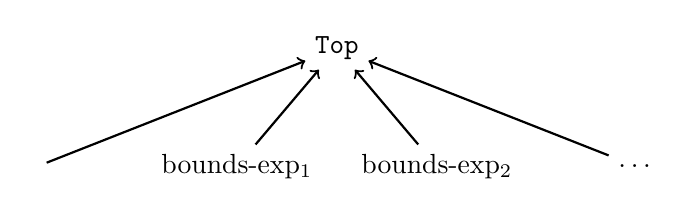
\begin{tikzpicture}[sibling distance=1in]
\node[rectangle, minimum size=8pt]{\texttt{Top}}
  child foreach \name in {\boundsnone, \var{bounds-exp\textsubscript{1}},
                          \var{bounds-exp\textsubscript{2}}, \ldots}
     {node{\name} edge from parent[<-, thick]};
\end{tikzpicture}
 
For an assignment to an \arrayptr\ variable, the existing
lattice value for the \arrayptr\ variable is killed, unless
the special conditions described in Section~\ref{section:extent-of-declarations}
are met. 
A new lattice value is generated for the \arrayptr\ variable. If the
assignment declares bounds for the \arrayptr\ variable, the new
lattice value is the bounds expression in the bounds declaration.
Otherwise, it is the value \boundsnone.

A declaration of a variable is handled similarly to an assignment,
except that there will not be any lattice value to kill. Lexical hiding
of variables involved in bounds declarations is not permitted. If the
declaration declares bounds for the \arrayptr\ variable, the
new lattice value is the bounds expression in the bounds declaration.
Otherwise, it is the value \boundsnone.

A variable going out of scope kills any existing lattice values in which
that variable occurs.

At control-flow split points, the lattice values for the
\arrayptr\ variables flow to all branches of the split. The
propagation is dataflow-sensitive but not control-flow sensitive. At
control-flow join points, the lattice values are unioned (moving upward
in the lattice). If the lattice values for an \arrayptr\
variable are not the same, the resulting value is \texttt{Top}.

\section{Bounds declarations and loops}

Loops often operate on variables declared outside of loops. They may
read the variables and then update the variables. When these variables
are \arrayptr\ variables they must have bounds and the bound
must be loop invariants.

The common case is that the bounds expression is invariant across all
iterations of the loop. The earlier \texttt{sum} example illustrates
this. The variable \texttt{current} is declared with bounds before a
loop. The loop modifies \texttt{current}, but the bounds for
\texttt{current} do not change:

\begin{verbatim}
/* sum integers stored between start and end, where end is not included */
int sum(array_ptr<int> start where start : bounds(start, end), array_ptr<int> end)
{ 
    int sum = 0;
    array_ptr<int> current : (start, end) = start;

    while (current < end) {
       sum = *current;
       current += 1; // bounds do not need to be redeclared here.
    }
}
\end{verbatim}

A programmer can declare bounds expressions that change on each
iteration of the loop. This may be necessary if an \arrayptr\
variable is modified to point to different memory during a loop
iteration. It also may be desirable for performance reasons. In either
case, there needs to be a loop-invariant bounds declaration.

The following example illustrates this. It is an implementation of
lexicographic comparisons of two arrays, using one pointer to scan each
array. The bounds at the variable declarations serve as loop invariant
bounds. The lower bounds for a variable are declared using the variable
itself, to reduce register pressure in the loop. This can enable
compilers to generate better code. Note that an optimizing compiler will
eliminate the runtime bounds checks easily.

\begin{verbatim}
/* lexicographic comparison of two arrays of integers */
int compare(array_ptr<int> x : bounds(x, x_end), 
            array_ptr<int> y : bounds(y, y_end)
            array_ptr<int> x_end,
            array_ptr<int> y_end)
{ 
    while (x < x_end && y < y_end) {
        if (*x == *y) {  // bounds check: x >= x && x < x_end; easily optimizable
                         // bounds check: y >= y && y < y_end; easily optimizable
            x++;
            y++;
        }
        else if (*x < *y) {  // bounds checks here are easily optimizable as well
            return -1;
        }
        else {
            return 1;
        }
    }
    if (x == x_end && y == y_end) {
        return 0;
    }
    else if (x != x_end) {
        return 1;
    }
    else {
        return -1; 
    }
}
\end{verbatim}

\section{Bundling statements and declarations}

Invariant bounds declarations must be valid at the end of every
statement. The effect of the statement must preserve the validity of the
bounds declarations. This is too restrictive when multiple statements
are used to update variables involved in a bounds declaration.

For example, suppose a function was added to the earlier sum example
that allowed for the buffer to be reallocated:
\begin{verbatim}
// external-scoped variables that hold a buffer and its length
int buflen = 0;
array_ptr<int> buf : count(buflen) = NULL;

int sum()
{
   int result = 0;
   for (int i = 0; i < buflen; i++) {
       result += buf[i]; // bounds checked
   }
   return result;
}

/* buggy resize function */
void resize(int len) 
{
    array_ptr<int> tmp : count(len) = malloc(sizeof(int) * len);
    copy(tmp, buf, buflen);
    buflen = len;  // fails at compile-time because the bounds are not true
    buf = tmp;
}
\end{verbatim}
In this example, the update to \texttt{buflen} fails compile-time
checking because the bounds declaration is not true after the
assignment. If the two updates are combined into one statement, though,
the checking would succeed.

\begin{verbatim}
void resize(int len) 
{
    array_ptr<int> tmp = malloc(sizeof(int) * len);
    copy(tmp, buf, buflen);
    buflen = len, buf = tmp; // succeeds, surprisingly
}
\end{verbatim}

This is an interesting difference between regular C, where

\begin{verbatim}
expr1, expr2;
\end{verbatim}

is always the same as:

\begin{verbatim}
expr1;
expr2;
\end{verbatim}

To allow invariant bounds to be checked after several statements or
initializing declarations, we introduce the notion of a bundled block.
Assignment statements and declarations can be grouped together using a
bundled block. Bounds declarations must be valid only at the end of the
block:

\begin{verbatim}
if (cond  && clen > 1) {
    bundle {
        c++;
        clen = clen - 1;
    }
}
\end{verbatim}

There is some subtlety with bundled blocks and function calls. The
bounds declarations for any static variables must be valid before any
function call in a bundle. This is because the called function may make
use of the static variables. It will assume that the bounds declaration
holds when it uses the static variables. In general, programmers may
deal with this requirement by using the idiom of storing function call
results in temporary variables and updating static variables \textit{en
masse} after the required function calls have been made.

The C syntax for is extended with:
\begin{tabbing}
\var{statement:}\=\\
\>\var{bundled-statement}\texttt{;} \\
\\
\var{bundled-statement:} \\
\>\texttt{bundled \{ \var{bundled-item-list\textsubscript{opt}} \}} \\
\\
\var{bundled-item-list:}\\
\> \var{bundled-item} \\
\> \var{bundled-item-list bundled-item} \\
\\
\var{bundled-item:}\\
\> \var{declaration}\\
\> \var{expression-statement} 
\end{tabbing}

\section{Bounds checks at pointer dereferences}
\label{section:bounds-checking-indirections}

Given *\var{e1}, where \var{e1} is an expression of type
\arrayptr, the compiler determines the bounds for \var{e1}
following the rules in Section~\ref{section:inferring-expression-bounds}.
Special rules are followed in
\texttt{bundled} blocks to determine the bounds for \var{e1}. The
compiler inserts checks before the memory pointed to by \var{e1} is
read or written that \var{e1} is non-null and that the value of
\var{e1} is in bounds.

If \boundsinfer{\var{e1}}{\bounds{\var{e2}}{\var{e3}}},
the compiler inserts a runtime check that \texttt{\var{e2} <= \var{e1} \&\&
\var{e1} < \var{e3}}. If the runtime check fails, the program
will be terminated by the runtime system or in, systems that support it,
a runtime exception will be raised.   If \boundsinfer{\var{e1}}{\boundscount{\var{e2}}},
this is expanded to \boundsinfer{\var{e1}}{\bounds{\var{e1}}{\var{e1} + \var{e2}}}
before inserting checks.  Of course a temporary variable would be used to hold the
value of \var{e1}.

If the default relative alignment has been overridden and
\boundsdecl{\var{e1}}{\boundsrel{\var{e2}}{\var{e3}}{\var{T}}}, the compiler checks whether
\texttt{sizeof(referent-type(\var{e1}))} is a common factor of \texttt{sizeof(\var{T})}. 
If it is, it inserts the same
runtime check as before. Otherwise, it inserts a runtime check that
\texttt{\var{e2} <= \var{e1} \&\& \var{e1} + sizeof(\var{T}) - 1 < \var{e3}}

Consider as an example, \verb|z = *x;| where 
\verb|x : bounds(x, x + c)|. The compiler will produce code of the form

\begin{quote}
\begin{verbatim}
dynamic_check(x != null);
dynamic_check(x <= x && x < x + c);
z = *t1;
\end{verbatim}
\end{quote}
The condition \texttt{x <= x} is trivially true. The
condition \texttt{x < x + c} simplifies to \texttt{0
< c}, that is \texttt{c > 0}, which is what one
would expect.

Now suppose pointer arithmetic is involved and \texttt{z = *(x + 5)}. The
bounds of \texttt{x + 5} will be the same as the bounds of \texttt{x}.
The expression \texttt{x + 5} must point into the same object as
\texttt{x} for this to be a valid memory access. This means that
\boundsdecl{\texttt{x + 5}}{\bounds{\texttt{x}}{\texttt{x + c}}}.
The compiler will produce code of the form:

\begin{quote}
\begin{verbatim}
dynamic_check(x != null);
t1 = x + 5;
dynamic_check(t1 != null && x <= t1 && t1 < x + c);
z = *t1;
\end{verbatim}
\end{quote}

Array subscripting works as expected. For \texttt{e1[e2]}, the
compiler computes the bounds of \texttt{e1}. The compiler inserts
runtime checks that \texttt{e1 + e2} is within this bounds. For example,
given \verb|x[5]| where \verb|x : bounds(x, x + c)|, the
compiler inserts runtime checks that \verb|x <= x + 5 < x + c|. 
The runtime checks simplify to \verb|5 < c|.

\subsection{Evaluation of bounds at bounds checks}

The preceding example raises a subtle point, which is when bounds
expressions are evaluated. Consider the following code:

\begin{verbatim}
array_ptr<int> x;
x = malloc ((sizeof(int) * 5)
where x : bounds(x, x + 5);
\end{verbatim}

When is \texttt{x + 5} evaluated?  In this design, 
the evaluation of a bounds expression in a bounds declaration is
{\em deferred} until a bounds check uses the bounds expression. 
This avoids the need for temporary storage to 
hold the value of \texttt{x + 5}.  The need for temporary storage would
be particularly problematic when bounds declarations are extended
to structures.   It also avoids complications when \texttt{x} is
\texttt{null}. Section~\ref{section:bounds-declarations-alternate-semantics} 
discusses eager evaluation of bounds expressions at
bounds declarations in more detail and explains why this was not chosen.

\section{Size computations and integer overflow or wraparound}
\label{section:integer-overflow-informal}

When objects are allocated dynamically in C, programmers have to compute
the amount of memory to allocate for the objects. It is well-known 
that integer overflow or wraparound in these computations can lead to buffer
overruns \cite{Howard2003,Mitre2015-128,Mitre2015-190,Mitre2015-680,Dietz2015}.
 In Checked C, the explicit size computations are not enough
to imply that the bounds for a newly-allocated object are valid.
Additional side conditions that deal with integer overflow or wraparound
are needed.

This section informally examines why and the additional conditions that
are needed. We start by looking at an allocation using malloc with an
old-style \texttt{char *} return type and a bounds declaration:

\begin{verbatim}
extern char *malloc(size_t s) : count(s);
\end{verbatim}

An array of type T is allocated with:

\begin{verbatim}
array_ptr<T> p : count(e1) = (arrayptr<T>) malloc(sizeof(T) * e1);
\end{verbatim}

The size computation in the count expression differs subtly from the
explicit computation on the right-hand side. In the count expression,
arithmetic with overflow checking is used, while the explicit
computation does not have overflow checking. Intuitively, this leads to
a mismatch when overflow or wraparound can happen, which causes static
checking to fail.

We expand the count expression to integer arithmetic to make its size
computation clear. \texttt{count(e1)} expands to \bounds{p}{p + e1}. 
Following the rules in Section~\ref{section:pointers-as-integers},
the expansion of \texttt{p +
e1} from pointer arithmetic to integer arithmetic depends on the type of
\texttt{e1}.

\begin{itemize}
\item
  If \texttt{e1} is an unsigned integer, \texttt{p + e1} expands to
  \texttt{p +\textsubscript{ovf} sizeof(T) *\textsubscript{ovf} e1}
\item
  If \texttt{e1} is a signed integer, \texttt{p + e1} expands to
  \texttt{p +\textsubscript{ovf} ((signed\_size\_t) sizeof(T))
  *\textsubscript{ovf} e1}.
\end{itemize}

The number of bytes added to \texttt{p} is the size computation of the
count expression. We can compare the size computations and see when the
values differ. We add casts for any implicit conversions that would
occur in the \texttt{malloc} size computation also:

\begin{longtable}[c]{lp{1.75in}p{1.75in}p{1in}}
\toprule
Type of e1 & Count size computation & \texttt{malloc} size computation &
Values differ?\tabularnewline
\midrule
\endhead
Unsigned integer & \texttt{sizeof(T) *\textsubscript{ovf} e1} &
\texttt{sizeof(T) * e1} & On overflow\tabularnewline
Signed integer & \texttt{((signed\_size\_t) sizeof(T))
*\textsubscript{ovf} e1} & \texttt{sizeof(T) * (size\_t) e1} & On
overflow or when \texttt{e1 <} 0.\tabularnewline
\bottomrule
\end{longtable}

For correctness, we want the count size computation and the
\texttt{malloc} size computations to produce identical values. This
implies that malloc did allocate the number of bytes expected by the
count size computation. We add conditions on \texttt{e1} to do this:

\begin{longtable}[c]{ll}
\toprule
Type of e1 & Restrictions\tabularnewline
\midrule
\endhead
Unsigned integer & \texttt{e1 <= UINT\_MAX/sizeof(T)}\tabularnewline
Signed integer & \texttt{e1 >= 0 and e1 <= INT\_MAX/sizeof(T)}\tabularnewline
\bottomrule
\end{longtable}

This has an interesting implication for any function that allocates an
array of \var{T}. If the count of elements is constant, of course these
conditions are trivial. If the count is non-constant, the function
must do the following checks:

\begin{itemize}
\item
  If the count is a signed integer, the function must check that the
  count \textgreater{}= 0 before trying to allocate the array.
\item
  If the size of \var{T} is larger than 1 byte, the function must check that the
  count is less than the upper bound as well.
\end{itemize}

When retrofitting existing code to use checked pointers, the code may be
unprepared for overflow or wraparound to happen during allocation. This
suggests that uses of \texttt{malloc} should be replaced by slightly
higher-level functions that takes the element count and the size of
elements and handle overflow. C already has a function that is suitable
for unsigned integer counts:

\begin{verbatim}
void *calloc(size_t nobj, size_t size);
\end{verbatim}

A signed version is needed too:
\begin{verbatim}
void *signed_calloc(signed_size_t nobj, size_t size);
\end{verbatim}
However, \texttt{calloc} also zeros the allocated memory.  For the sake of efficiency,
new allocation functions that compute sizes but do not zero memory may be needed.